\chapter{Introduction}
\label{chapter:introduction}
With the advent of the Web, the world has seen a deluge of digital text.  
Word Sense Disambiguation(WSD) is a notoriously difficult problem in understanding text. Ambiguity is very common in text but humans are so competent at figuring out the word sense from context that most of the time they do not notice the ambiguity in the meaning of the word. Accurate sense disambiguation would aid a number of Natural Language applications; however it is widely acknowledged by WSD researchers that current accuracy levels of WSD systems need to be improved before they can be practically used in applications \citep{ide2006making}.

There are two major problems faced by the researchers in this area. One major problem is the dearth of sufficient training data for supervision. With a handful of sense-tagged texts currently available, existing WSD systems do not have examples for all the senses of a word most of the times. The other major problem that automatic disambiguation systems face is the fine-grained nature of the sense-distinctions in the sense inventory, WordNet in particular. 

WordNet \citep{miller1995wordnet} \citep{fellbaum1998wordnet} is well known to the Natural Language Processing community as a valuable resource and is one of the most widely used lexical resources. WordNet being a fine grained sense inventory makes it hard even for humans to reliably and consistently distinguish among word senses. In this thesis we would be addressing the latter problem and produce graded word sense relationships which can be used to derive coarse sense clusters with required granularity.

\section{Motivation}
The motivation for the work is two-fold: the variable needs of sense granularities by applications and saturation in fine-grained WSD performance.

\subsection{Different granularity requirements of different tasks}
The applicability of the work stems from the fact that different tasks and applications require different granularities of sense distinctions. The subtleties of sense distinctions captured by WordNet are helpful for language leaners \citep{snow07mergesense} and in machine translation of languages as diverse as Chinese and English \citep{Ng:2003}. 

On the other hand, for tasks like Document Categorization \citep{buitelaar2000reducing} and Query Expansion \citep{moldovan2000using}, it may be sufficient to know if a given word belongs to a coarsely defined class of WordNet senses. Using fine grained sense inventory of WordNet may be detrimental to the performance of the performance of these applications. Thus developing a framework which can generate inventories with different granularities is a crucial task.

\subsection{Saturation in Fine-Grained WSD}%??? and scope of improvement by coarsening senses
Lets observe the inter-tagger agreement(ITA) estimates of the data preparation for the Senseval/SemEval tasks on WSD: All Words(AW) or Lexical Sample(LS) in table \ref{tab:itaWSD}.

\begin{center}
\begin{longtable}{| c | c | c | c | c | c |}      
    \hline
Workshop and Task & WordNet Version & Verb & Noun & Adjective & Overall \\\hline 
Senseval-2 AW\footnote{Only approximate information on ITA is available} & \multirow{2}{*}{1.7} & \multirow{2}{*}{70-80} & \multirow{2}{*}{NA} & \multirow{2}{*}{NA} & \multirow{2}{*}{NA} \\ 
\citep{Senseval2AllWordsTask} & & & & & \\ \hline

Senseval-2 LS & \multirow{2}{*}{1.7} & \multirow{2}{*}{NA} & \multirow{2}{*}{86.3} & \multirow{2}{*}{83.4} & \multirow{2}{*}{NA} \\ 
\citep{Senseval2LexicalSampleTask} & & & & & \\ \hline

Senseval-3 AW  & \multirow{2}{*}{1.7.1} & \multirow{2}{*}{67.8} & \multirow{2}{*}{74.9} & \multirow{2}{*}{78.5} & \multirow{2}{*}{72.5}\\ 
\citep{Senseval3AllWordsTask} & & & & & \\ \hline

Senseval-3 LS & \multirow{2}{*}{1.7.1} & \multirow{2}{*}{NA} & \multirow{2}{*}{NA} & \multirow{2}{*}{NA} & \multirow{2}{*}{67.3}\\ 
\citep{Senseval3LexicalSample} & & & & & \\ \hline

Semeval 2007 AW & \multirow{2}{*}{2.1} & \multirow{2}{*}{72} & \multirow{2}{*}{86} & \multirow{2}{*}{NA} & \multirow{2}{*}{NA} \\ 
\citep{Semeval2007WSD} & & & & & \\ \hline
\caption{Inter-tagger agreement for Various Data Preparations} 
\label{tab:itaWSD}
\end{longtable}
\end{center}

It is a generally agreed upon fact that ITA serves as an upper bound on the performance of WSD systems. \citep{Navigli06meaningfulclustering} estimates that unrestricted fine-grained WSD performance has a 70\% upper bound.  From Senseval and SemEval worskshops we observe that state-of-the-art automatic disambiguation systems indeed are not able to beat this bound. Therefore it seems that the major bottleneck in effective sense disambiguation is the fine grained nature of WordNet.

The above points are substantiated by the ITA achieved in preparation of gold standard datasets and performance of the systems in SemEval-2007 Task on Coarse grained WSD \citep{navigli-litkowski:SemEval-2007}. The ITA values on train and test datasets were 86.44\% and 93.80\%. These figures, compared to those in the table \ref{tab:itaWSD}, show that the performance of the WSD systems can be improved by changing the granularity of the adopted sense inventory.

Some of the best systems of SemEval-2007 Coarse Grained WSD task achieved performances in the early 80s in the all words task and in the high 80s for the lexical sample task as compared to previous Senseval evaluation exercises, where state-of-the-art systems achieved performance far below 70\%. This encourages us to study in depth the ideas for good sense clustering algorithms and use them to improve the WSD systems so that they can be used in practical scenarios.

\begin{comment}
To understand the granularity of WordNet, lets take an example.
\begin{example}
Consider the senses of the word \textit{evidence} as a \textit{noun} from WordNet version 3.1\footnote{Online WordNet Search: \url{http://wordnetweb.princeton.edu/perl/webwn}} in the table \ref{tab:evidenceExample}.
For most of the applications the sense distinctions are too-fine and are not required. 
One might say that they are all clearly related. \cite{mccarthy2006relating}
\begin{table}[h]
\centering
\begin{tabular}{ | l | p{12cm} |} 
\hline
WordNet Sense & Gloss \\ \hline
evidence\#n\#1 & evidence, grounds (your basis for belief or disbelief; knowledge on which to base belief)  ``the evidence that smoking causes lung cancer is very compelling`` \\ \hline
evidence\#n\#2 & evidence (an indication that makes something evident) ''his trembling was evidence of his fear'' \\ \hline
evidence\#n\#3 & evidence ((law) all the means by which any alleged matter of fact whose truth is investigated at judicial trial is established or disproved) \\ \hline    
\end{tabular}
\caption{Senses of the word \textit{evidence}} 
\label{tab:evidenceExample}
\end{table}
\end{example}
\end{comment}

\section{WordNet}
WordNet is a Lexical Knowledge Base (LKB) for the English language. The project was begun by George Miller, and is currently being maintained at Princeton University. WordNet is divided into 4 broad hierarchies based on POS, one each for nouns, verbs, adjectives and adverbs. WordNet is similar to a thesaurus in the sense that synonymous word senses are grouped together into a single concept called {\em synset}. Every synset is described by a brief definition.

Synsets in WordNet are connected by relations, which can be categorized into two kinds:
\begin{itemize}
 \item \textbf{Lexical Relations:} These are connections between word senses contained in respective synsets.
 \begin{itemize}
  \item Antonymy: Synset A is an antonym of synset B if A and B have senses of opposite meaning.
  \item Pertainymy: Adjective A is related to noun B by this relation if A ``pertains to'' B.  
  \item Nominalization: Noun A is related to verb B by this relation if A ``nominalizes'' B.
 \end{itemize}
 \item \textbf{Semantic Relations:} These are connections between synsets as a whole.
 \begin{itemize}
  \item Hypernymy: Synset A is a hypernym of synset B if B is a ``kind of'' A.
  \item Hyponymy and Troponymy: Hyponymy is the inverse relation of hypernymy for nouns, while troponymy is the inverse relation of hypernymy for verbs.
  \item Meronymy: Synset A is a meronym of synset B if A is a ``part of'' B.
  \item Holonymy: The inverse relation of meronymy.
  \item Entailment: Verb A entails verb B if A follows B.
  \item Similarity: Relates similar adjectives.
  \item Atribute: Noun A is related to adjective B by this relation if A serves as an attribute of B.
  \item See also: Applicable if two adjectives are ``related'' semantically.
 \end{itemize}
\end{itemize}

Figure \ref{fig:excerptFromWordNet} shows a subgraph of WordNet \citep{navigli2009WSDSurvey}. WordNet 3.0 contains 155,287 words organized into a total of 117,659 synsets. \footnote{\url{http://wordnet.princeton.edu/man/wnstats.7WN.html}}

\begin{figure}[h]
\begin{center}
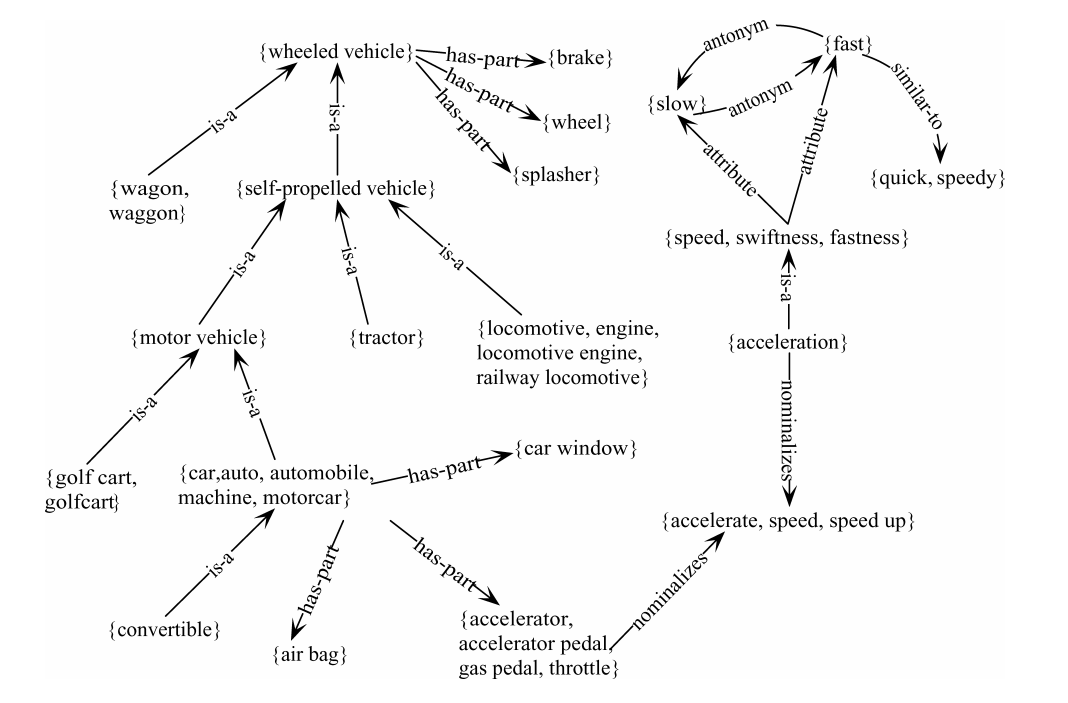
\includegraphics[scale = 0.6]{excerptFromWordNet.png}
\caption{Excerpt From WordNet}
\label{fig:excerptFromWordNet}
\end{center}
\end{figure}

\section{Problem Statement}
Formally, the task we are attempting has two objectives: 
\begin{enumerate}
\item Given a fine-grained sense inventory like WordNet, we wish to produce a clustering over WordNet synsets at any arbitrary granularity, which can serve as a coarse sense dictionary. 
\item Given a coarse sense inventory obtained by clustering fine-grained senses, assess its quality and show that it helps improve sense disambiguation on standard test sets.
\end{enumerate}

\section{Related Work}
\label{chapter:Background}
Systems using WordNet as the underlying ontology often suffer because of the fine-grained nature of the sense inventory. With more and more applications using WordNet, clustering word senses such that the application developer has the control over the granularity becomes very important.

\paragraph{}
One of the earliest attempt at coarsening of Machine Readable dictionaries was made by \citep{Dolan:1994}. 
They tried to discover similarities between senses of Longman's Dictionary of Contemporary English(LDOCE) using multiple heuristics based on a variety of information about a sense's meaning.

\paragraph{}
A wide variety of automatic methods have been proposed since then for coarsening fine-grained inventories. In this section, we discuss the approaches proposed in literature to coarsen sense inventories. The different ideas to cluster senses can be broadly categorized as follows: 
\begin{itemize}
\item Merging senses based on the sense ontology structure.
\item Clustering based on word sense similarity estimated from external corpora.
\item Exploiting Disagreements: between human annotators or between WSD systems.
\item Using translational equivalences of word senses.
\item Mapping to coarser sense inventories.
\item Clustering senses using supervision.
\end{itemize}

\subsection{Merging senses based on ontology structure}
\citep{peters1998automatic} suggest merging of two word senses based on structural cues derived from the ontology structure. They cluster senses which are connected by ontology based relations like  \textit{twins}\footnote{Two synsets having more than one word common.}, \textit{autohyponymy}\footnote{If one sense is a direct descendant of the other in the hypernym-hyponym ontology.}, 
\textit{sisters}\footnote{Word senses that share the same hypernym}, 
\textit{cousins}\footnote{Node pairs whose hyponyms exhibit a specific relation to each other: identified and listed by lexicographers in WordNet 1.5.} etc.
\citep{Mihalcea01ez.wordnet:principles} extended this idea and proposed six semantic principles to merge synsets and probabilistic principles to drop infrequent synsets.
Some interesting principles include merging synsets sharing a \textit{pertainym}, \textit{antonym} or sharing the same \textit{verb group}\footnote{Verb Groups are manually determined by lexicographers.}.
This was the first attempt to group synsets instead of word senses.

\paragraph{}
A number of synset similarity measures based on the WordNet structure have also been proposed in literature like 
Path Based Similarity Measures by \citep{WuPalmer:1994}, \citep{LCH:1998}, Information Content Based Measures by \citep{Resnik:1995}, \citep{JCN:1997}, \citep{Lin:1998} and Gloss Based Heuristics by \citep{Lesk:1986},\citep{Banerjee:2002}. We discuss these similarity measures in detail in Section \ref{section:similarityMeasures}.
Though these measures have not been used directly for WordNet sense clustering, they have motivated researchers in the NLP community to make full use of the WordNet structure to capture similarity between senses.

\subsection{Clustering based on Word Sense similarity estimated from External Corpora}
For estimating similarity between words, many corpus oriented attempts have been made like \citep{Pereira:93a}, \citep{Lin:1998}, \citep{kolb2008disco} and \citep{agirre2009study}. The problem with these approaches is that they are not able to handle the polysemous nature of words. Also, the dearth of sense annotated corpora prevents most of these methods to be used effectively in computing word sense similarities.

\paragraph{}
\citep{agirre2003clustering} associated a topical vector with each word sense, called \textit{Topic Signature}, which captures the relatedness between the target word sense and vocabulary. The cosine similarity between the vectors of two senses is used as the similarity between them. To calculate these vectors, they collect contexts for a polysemous words from manually sense-tagged corpora and by using instances of a polysemous word's monosemous relatives\footnote{Single-sense synsets related by hyponym, hypernym or any other relation of WordNet.} from large untagged corpora and the web. The idea behind the approach is that because of lack of sense annotated data, semantically close senses may not have a lot of direct shared contexts, but they are expected to have similar distributional neighbours.

\paragraph{}
On similar lines is the approach by \citep{mccarthy2006relating}. They calculate sense similarities using a combination of the JCN WordNet based similarity measure \citep{JCN:1997} and word-to-word distributional similarity. They introduce a more relaxed notion of sense relatedness which allows the user to control the granularity for the application in hand.

\subsection{Exploiting Disagreements: between WSD Systems or between Human Annotators}
The central idea involved here is that whenever good WSD systems or human annotators get confused while disambiguating, the senses they mark as answers are semantically related to the correct answer.
\begin{example} 
\label{example:fish}
Consider the following noun senses of the word \textit{fish}, taken from WordNet 3.1:
\begin{itemize}
\item fish (any of various mostly cold-blooded aquatic vertebrates usually having scales and breathing through gills) ``the shark is a large fish"

\item fish (the flesh of fish used as food) ``in Japan most fish is eaten raw"

\item Pisces, Fish ((astrology) a person who is born while the sun is in Pisces)

\item Pisces, Pisces the Fishes, Fish (the twelfth sign of the zodiac; the sun is in this sign from about February 19 to March 20)
\end{itemize}
\end{example}

It is unlikely that a human annotator mistags the astrology sense of the word \textit{fish} with its food sense. Similar results are expected from a good WSD system as well.

\paragraph{}
\citep{chklovski2003exploiting} derives confusion matrices exploiting the disagreements between human annotators and uses the same to generate coarse sense clusters. On the other hand, \citep{agirre2003clustering} uses the publicly available outputs of Senseval-2 \citep{Edmonds:2001} participants to construct the confusion matrices between word senses and then cluster them using hierarchial agglomerative clustering. Dearth of available manually sense-tagged data and not-so-high performance of the WSD systems limits the applicability of the above mentioned ideas.

\subsection{Using translational equivalences of word senses}
\citep{chugur2002polysemy} constructed similarity matrices for Senseval-2 \citep{Edmonds:2001} words based on translations of these words in four languages. The principle involved can be summed as: \textit{two word senses which are translated with the same word sense in other language are expected to be semantically similar}. Using multiple languages enables us to cover all the sense divisions offered by different languages. \citep{agirre2003clustering} uses the similarity matrices provided by \citep{chugur2002polysemy} and report resulting hierarchial clusters.

With the advent of WordNets being developed in multiple languages\footnote{GlobalWordNet lists the WordNets available in the public domains: \url{http://www.globalwordnet.org/gwa/wordnet_table.html}.} as well as multilingual ontologies like BabelNet \citep{NavigliPonzetto:12aij}, this seems a promising area which can help in coarsening of senses.


\subsection{Mapping to coarser sense inventories}
Mapping WordNet to other inventories either manually or automatically to generate coarse senses has also been tried by many researchers in the NLP community. When the different WordNet senses map to the same sense in the other ontology via manual mapping or automatic mapping, it is expected that the senses must have been semantically close. The underlying assumption being that the automatic mapping is able to capture the semantic similarity between the concepts in both the ontologies with high efficacy.

The attempts made in this direction include mapping WordNet to Hector Lexicon \citep{palmer2007making}, PropBank \citep{palmer2004different} and Levin Classes \citep{levin1993english} \citep{palmer2007making}. Most of these mappings are not complete in both directions, which hampers their utility.

The automatic approach presented by \citep{Navigli06meaningfulclustering} for mapping between sense inventories, WordNet to Oxford English Dictionary to be precise, is an elegant approach exploiting similarities in glosses and semantic relationships in the sense inventories. The approach can be extended to discover more semantic relationships in WordNet by using the ontology structure of the ontology mapped to WordNet.

\subsection{Clustering senses using supervision}
One of the earliest attempt to cluster senses using supervision was proposed by \citep{snow07mergesense}. They train a Support Vector Machine \citep{vapnikSVM:95} using features derived from WordNet and other lexical resources, whose predictions serve as a distance measure between synsets. For synset pairs with no common words, they assume a zero sense similarity score. They cluster synsets using average link agglomerative clustering and the synset similarity model learnt. While merging synsets to construct a coarse taxonomy, the merged synset inherits its hypernymy from its most frequent constituent sense. All other relationships are added to the new merged sense as long as the acyclic nature of the relations is conserved.

\section{Discussion}
In this section, we discuss some ideas which shaped the direction of our approach to the problem of WordNet sense clustering.

\subsection{Dropping Infrequent WordNet Synsets}
To reduce polysemy in WordNet, \citep{Mihalcea01ez.wordnet:principles} proposed to drop infrequent synsets, along with merging similar senses. They scored the synsets using frequency information of senses in SemCor \citep{SemCor} and dropped the low scoring synsets. 

We study the usefulness of this idea on the SemEval 2007 WSD test datasets \citep{navigli-litkowski:SemEval-2007}, in which we have three generic Wall Street Journal texts and two domain-specific documents (relating to computer programming and Italian painting respectively). Our scoring function is similar to the one proposed by \citep{Mihalcea01ez.wordnet:principles} and is given by:

\begin{equation}
Score(Synset) = \sum_{i \in Synset} Score(WordSense_i) 
\end{equation}

\begin{equation}
Score(WordSense) = \frac{Frequency(WordSense)+\alpha}{Frequency(LemmaWord) + \alpha*NumberOfSenses(LemmaWord)} 
\end{equation}

Here $\alpha$ is the Laplacian correction parameter(for our study we take $\alpha=1$).
The scoring function does not make reference to the component word senses directly and thus we do not have to deal with the data sparseness issue that arises from the limited size of the corpus.

We drop the synsets whose score is less than a threshold and study the number of instances for which the correct answer was removed, thus accounting for error. Since the task was on coarse grained WSD evaluation, we have multiple senses as the correct answer. In this case, we measure the fraction of senses removed from the set of correct senses for each of the instances. We report the error score calculated, weighted by the number of instances in the documents.

% \begin{center}
% \begin{longtable}{| c | c | c |}  
% \hline
% \textbf{Corpora Type} & \textbf{Threshold} & \textbf{Weighted Error Score} \\ \hline
% WSJ & 0.03 & 7.72 \\ \hline
% Domain & 0.03 & 10.48 \\ \hline
% WSJ & 0.06 & 13.91 \\ \hline
% Domain & 0.06 & 14.19 \\ \hline
% WSJ & 0.1 & 18.77 \\ \hline
% Domain & 0.1 & 19.13 \\ \hline
% \caption{Synsets Dropping Study}
% \label{tab:synsetsDroppingStudy}
% \end{longtable}
% \end{center}

\begin{center}
\begin{longtable}{cc|c|c|c|c}
\cline{3-5}
& & \multicolumn{3}{ c| }{Threshold} \\ \cline{3-5}
& & 0.03 & 0.06 & 0.1 \\ \cline{1-5}
\multicolumn{1}{|c }{\multirow{2}{*}{Corpora} } & \multicolumn{1}{ |c| }{WSJ} & 7.72 & 13.91 & 18.77 \\ \cline{2-5}
\multicolumn{1}{|c }{} & \multicolumn{1}{ |c| }{Domain} & 10.48 & 14.19 & 19.13 & \\ \cline{1-5}
\caption{Dropping Infrequent Synsets - A Comparision} 
\label{tab:synsetsDroppingStudy}
\end{longtable}
\end{center}


We observe that for lower thresholds, the error rate is higher for domain specific datasets whereas as we increase the threshold, thus removing more and more synsets, the error rates of both the datasets become comparable. The results match our expectation as we expect that some of the words in domain specific datasets would have low frequencies and thus low scores. To summarise, while working with text from the general domain, removing some infrequent synsets might improve the disambiguation but in case of domain specific datasets, it should not be done.

\subsection{Clustering Synsets Vs Clustering Senses}
For generating a coarse sense inventory, many researchers have focused on clustering WordNet senses into groups i.e. generate coarse senses for each word by merging its senses \citep{agirre2003clustering} \citep{chklovski2003exploiting} \citep{Navigli06meaningfulclustering}. In this approach, we would like to highlight two problems. One problem is that it requires a stopping criterion for each word such as the number of final classes. In literature, researchers have used the numbers determined by the available gold standard datasets for the purposes of evaluation \citep{agirre2003clustering}. As the right number of classes for each word cannot usually be predetermined even if the application is known, such coarsening systems cannot be used to derive coarse senses for all the words. The other problem is the inconsistent sense clusters obtained because of independent generation of coarse senses for each word. Even manually done sense clusterings can have this error: consider the sense groupings of the verbs \
textit{need} and \textit{require} from Senseval-2 judgements in figure \ref{fig:transitiveError} \citep{snow07mergesense}.

\begin{figure}[h]
\begin{center}
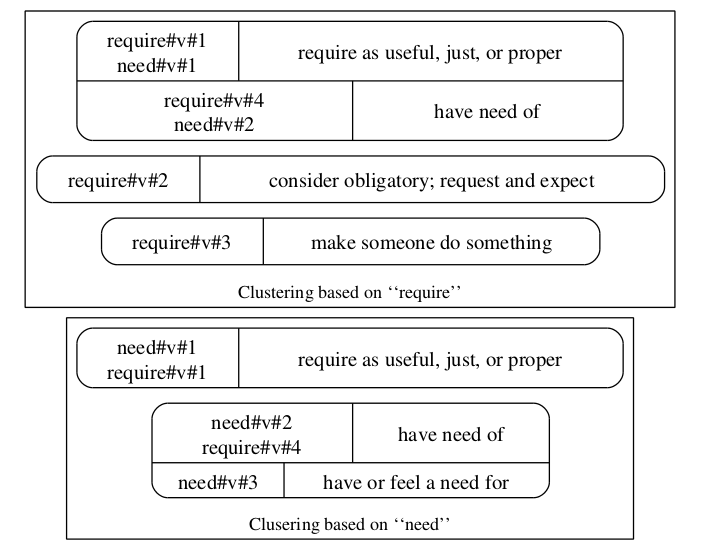
\includegraphics[scale = 0.6]{transitiveError.png}
\caption{Inconsistency in sense groupings for the verbs \textit{need} and \textit{require} from Senseval-2 judgements}
\label{fig:transitiveError}
\end{center}
\end{figure}

The two WordNet 2.1 senses \textit{need\#v\#1} and \textit{need\#v\#2} clustered in word specific labelling for \textit{require}, are not clustered in word specific labelling for \textit{need}. These transitive closure errors suggest that for deriving consistent coarse senses, we should cluster synsets and not senses.

\section{Evolution of Evaluation Frameworks}
We would like to highlight here the different frameworks used in literature for evaluating the sense clustering problem. Early systems studied the quality of clusters of word senses by studying polysemy degree of the text \citep{Mihalcea01ez.wordnet:principles} or by measuring the entropy and purity of the clusters obtained \citep{agirre2003clustering}.

Another idea is to compare the clustering obtained against a manually sense clustered dataset as done by \citep{chklovski2003exploiting}. This can be done by treating clustering as a pairwise classification task and reporting the F-Score for the classification task. The problem with this approach of evaluation is that the number of intra-cluster pairs is often small compared to inter-cluster pairs in clustering tasks. This imbalance could lead to understating pairwise similarity and can be avoided by using FScore for both the classes as performance evaluators.

The recent line of thought in evaluation is to go for a task based evaluation. \citep{mccarthy2006relating} studied the performance of first sense heuristics in the Senseval-2 English LS Task \citep{Senseval2LexicalSampleTask}. \citep{Navigli06meaningfulclustering} and \citep{snow07mergesense} assess the effect of automatic sense clustering on the three best-ranking WSD systems of the English AW task at Senseval-3 \citep{Senseval3AllWordsTask}. Since the main motive for coarsening WordNet inventory is to make WSD a plausible task, studying the performance of sense disambiguation systems on automatically generated coarsened senses seems a well founded approach.

\section{Broad Overview of our Approach}
We propose a framework which derives a coarse sense inventory by learning a synset similarity metric. We focus on the coarsening of noun synsets of WordNet and show that the coarse-grained sense inventory obtained notably improves the disambiguation of nouns.

Our approach closely resembles \citep{snow07mergesense} as far as supervised learning of the synset similarity is concerned. But to learn synset similarity of synset pairs which don't share a word, instead of giving them zero similarity, we learn it using a variant of the SimRank framework \citep{Jeh02simrank}. 

Also, \citep{snow07mergesense} proposes to modify the WordNet ontology structure to produce a coarse version of WordNet; however we argue on the lines of \citep{mccarthy2006relating} that a softer notion of relationships between senses should be used compared to fixed groupings so that the variable granularity needs of different applications can be met.

\begin{comment}
\subsection{Understanding sense clustering}
When we merge two synsets, should we modify the underlying structure of taxonomy as well?
What should be the repercussion of the mergings on the taxonomy?

An important point to note here is that if we merge two synsets and introduce the merged synsets instead of the original synsets in the WordNet taxonomy, either we'll be adding some spurious relations and/or we'll be losing some relationship information.

\end{comment}

\section{Organization of Thesis}
In this chapter, we introduced the problem, reviewed the algorithms proposed for the task of sense clustering and the evaluation frameworks for the same. 
The rest of this thesis is organized as follows. 
Chapter \ref{chapter:SupervisedSynsetSimilarity} discusses a supervised attempt to capture WordNet synset similarity using various features derived from WordNet and external corpora. 
Chapter \ref{chapter:Semi-SupervisedSynsetSimilarity}, presents a semi-supervised approach to estimate WordNet synset similarity using a variant of SimRank \citep{Jeh02simrank} and describes our approach to produce a coarse sense inventory. 
The conclusions and future work are part of chapter \ref{chapter:conclusion}.
